% Relatório em LaTeX para o trabalho de PPC Autor: Daniel Martins Cabrita de
% Sousa Data: Outubro 2025
\documentclass[a4paper,openright,twoside,11pt]{report}

% Packages utilizadas e respetivos parâmetros.
\usepackage[utf8]{inputenc}
\usepackage[english]{babel}

\usepackage{lipsum} % gerador de texto
\usepackage{graphicx}
\usepackage{url}
\usepackage[Algoritmo]{algorithm}
\usepackage{algorithmicx}
\usepackage{algpseudocode}
\usepackage{acronym}

\usepackage{listings}
\usepackage{xcolor}

% Definições das dimensões das páginas
\setlength{\textheight}{24.00cm}
\setlength{\textwidth}{15.50cm}
\setlength{\topmargin}{0.35cm}
\setlength{\headheight}{0cm}
\setlength{\headsep}{0cm}
\setlength{\oddsidemargin}{0.25cm}
\setlength{\evensidemargin}{0.25cm}

%\renewcommand{\baselinestretch}{1}

% Página inicial (capa)
\title{
   \vspace{-50mm}
   \begin{minipage}[l]{\textwidth}
      \hspace{-20mm}\resizebox{75mm}{!}{
\includegraphics{images/fcul.png}}\\
   \end{minipage}\\[20mm]
   \textbf{Assignment \#1} 
   \\ 
   Knapsack Problem \\ Parallel and Concurrent Programming 
}

% Nome dos autores (um por linha)
\author{
\begin{tabular}{ll}
             & Daniel Martins Cabrita de Sousa: 66128  \\
\end{tabular}}

\date{
\begin{tabular}{ll}
  {Professor:} & Wellington Júnior \end{tabular}\\[10mm]
Assignment report for Parallel and concurrent programming \\
MSc in Software Engineering \\ [50mm] October 2025}


\begin{document}
\pagenumbering{roman}
\thispagestyle{empty}
\maketitle

\baselineskip 18pt 
\newpage
\thispagestyle{empty}
% Fim da contracapa

% Reiniciar a numeração de páginas
\setcounter{page}{1}
\pagenumbering{arabic}

\chapter{Introduction} \label{cap:intro}

This report presents the implementation and analysis of parallel approaches to solving the Knapsack Problem using Genetic Algorithms in Java. The assignment evaluates understanding of Java's threading model, thread lifecycle, and synchronization primitives.

\section{Problem Context}

The Knapsack Problem is a fundamental optimization problem in computer science. Due to the exponential computational cost of evaluating all possible item combinations, heuristic methods like Genetic Algorithms are often employed to find near-optimal solutions efficiently.

\section{Objectives}

The primary objective is to explore different parallelization strategies to improve performance while maintaining correctness. Key areas for parallelization include fitness evaluation, genetic operations, and population management. A critical constraint is preserving the single print output per generation from the original sequential implementation.

\chapter{Implementation} \label{cap:implementation}


In this assignment, three distinct parallelization strategies were implemented:

\begin{enumerate}
    \item \textbf{Master-Worker Pattern with Poison Pill}
    \item \textbf{Scatter-Gather Pattern}
    \item \textbf{Fork-Join Pattern}
\end{enumerate}

All these strategies apply parallelization to each generation step of the
algorithm, specifically targeting the methods that evaluate the fitness of
individuals in the population. This focus is strategic since fitness evaluation
is the most computationally intensive task and benefits significantly from
parallel execution.

\section{Master-Worker Pattern with Poison Pill} \label{sec:master-worker}

The Master-Worker uses a master thread to be responsible for distributing tasks
to multiple worker threads. This implementation creates a thread pool with a
configurable number of workers (\texttt{maxThreads} parameter, defaulting to
\texttt{Runtime.getRuntime().availableProcessors()}). The master divides the
population into equal chunks based on a calculated chunk size (\texttt{POP\_SIZE
/ maxThreads}), ensuring balanced workload distribution among workers. \\
\\
The implementation consists of three key components:

\subsection{Core Classes}

\begin{itemize}
    \item \texttt{Worker} class that implements \texttt{Runnable} - represents a
    worker thread that continuously polls the task queue for work
    \item \texttt{Task} class - encapsulates the work to be performed,
    containing a \texttt{TaskType} and a \texttt{Runnable} with the actual logic
    \item \texttt{TaskType} enum - distinguishes between regular tasks
    (\texttt{RUNNABLE}) and termination signals (\texttt{POISON\_PILL})
\end{itemize}

\subsection{Architecture}
The master maintains a thread-safe \texttt{LinkedBlockingQueue<Task>} that
serves as the communication channel between the master and workers. Workers are
initialized once at the beginning of the algorithm and remain active throughout
all generations, continuously processing tasks as they become available.

\subsection{Parallelized Operations}
This pattern is applied to four critical algorithm operations:

\begin{enumerate}
    \item \textbf{Fitness Calculation} (\texttt{calculateFitness()}): Each
    worker evaluates the fitness of individuals in its assigned chunk of the
    population
    \item \textbf{Best Individual Selection} (\texttt{bestOfPopulation()}):
    Workers find the best individual in their chunk using
    \texttt{AtomicReference} with compare-and-swap operations to safely update
    the global best
    \item \textbf{Population Reproduction} (\texttt{calculateBestPopulation()}):
    Workers perform tournament selection and crossover operations to generate
    new individuals
    \item \textbf{Mutation} (\texttt{mutate()}): Workers apply mutation to
    individuals in their assigned range based on the mutation probability
\end{enumerate}

\subsection{Synchronization}
Each parallelized step utilizes a \texttt{CountDownLatch} initialized with the
number of workers. As each worker completes its assigned chunk of work, it calls
\texttt{countDown()}, while the master waits using \texttt{await()} before
proceeding to the next step. This mechanism ensures proper synchronization
between generations.

\subsection{Lifecycle Management}
Workers are initialized once at the beginning (\texttt{startWorkers()}) and
terminated at the end by enqueueing a poison pill for each worker
(\texttt{stopWorkers()}). This approach minimizes thread creation overhead and
maintains consistent performance across generations.

\newpage

\section{Scatter-Gather Pattern}\label{sec:scatter-gather}

The Scatter-Gather pattern divides the population into smaller chunks
(scattered) across multiple threads for parallel processing, then collects the
results (gathered) after completion. This implementation utilizes Java's
\texttt{ExecutorService} with a fixed thread pool to manage parallel execution
efficiently.

\subsection{Core Architecture}

\begin{itemize}
    \item Uses \texttt{Executors.newFixedThreadPool(maxThreads)} where
    \texttt{maxThreads} is a configurable parameter (defaulting to
    \texttt{Runtime.getRuntime().availableProcessors()})
    \item Employs a centralized \texttt{computeFutures()} method that handles
    the scatter-gather logic for all parallelized operations
    \item Creates \texttt{Future} objects to track and synchronize the
    completion of parallel tasks
\end{itemize}

\subsection{Scatter Phase}
The \texttt{computeFutures()} method divides the work range into equal chunks
based on \texttt{chunkSize = total operations / maxThreads}. Each thread
receives a specific range to process:

\begin{itemize}
    \item Thread 0: processes indices \texttt{[start, start + chunkSize)}
    \item Thread 1: processes indices \texttt{[start + chunkSize, start + 2 *
    chunkSize)}
    \item Last thread: processes remaining indices to handle any remainder from
    integer division
\end{itemize}

\subsection{Gather Phase}

After submitting all tasks to the thread pool, the method calls
\texttt{futures.forEach \{ it.get() \}} to wait for all threads to complete
their work before proceeding. This ensures synchronization between parallel
operations.

\subsection{Parallelized Operations}\label{sec:scatter-gather-operations}

\begin{enumerate}
    \item \textbf{Fitness Calculation} (\texttt{calculateFitness()}): Each
    thread evaluates fitness for individuals in its assigned range
    \item \textbf{Best Individual Selection} (\texttt{bestOfPopulation()}):
    Threads find local best individuals and use \texttt{AtomicReference} with
    compare-and-swap to update the global best
    \item \textbf{Population Reproduction} (\texttt{calculateBestPopulation()}):
    Each thread performs tournament selection and crossover for its assigned
    range
    \item \textbf{Mutation} (\texttt{mutate()}): Threads apply mutation to
    individuals in their assigned range based on mutation probability
\end{enumerate}

\subsection{Thread Management}
The thread pool is created once per algorithm execution and reused across all
generations, minimizing thread creation overhead. The pool is properly shut down
in a \texttt{finally} block to ensure resource cleanup.

\section{Fork-Join Pattern}

The Fork-Join pattern utilizes Java's Fork-Join framework to recursively divide
tasks into smaller subtasks until they reach a manageable size (threshold), then
processes them in parallel and combines the results. This implementation
leverages \texttt{ForkJoinPool} and \texttt{RecursiveAction} to achieve
work-stealing parallelism.

\subsection{Core Architecture}

\begin{itemize}
    \item Utilizes \texttt{ForkJoinPool(maxThreads)} where \texttt{maxThreads}
    is a configurable parameter (defaulting to
    \texttt{Runtime.getRuntime().availableProcessors()})
    \item Implements \texttt{RecursiveAction} for each algorithm operation
    requiring parallelization
    \item Employs a configurable threshold (default 1000) to determine when to
    stop subdividing tasks
    \item Uses \texttt{invokeAll()} to fork subtasks and automatically join
    their results
\end{itemize}

\subsection{Fork Phase (Task Subdivision)}
The \texttt{computeRange()} method implements the recursive subdivision logic:

\begin{itemize}
    \item If the work range \texttt{(end - start)} is smaller than or equal to
    the threshold, executes the task directly
    \item Otherwise, splits the range in half at the midpoint: \texttt{mid =
    (start + end) / 2}
    \item Creates two \texttt{RecursiveAction} subtasks: left half
    \texttt{[start, mid)} and right half \texttt{[mid, end)}
    \item Uses \texttt{invokeAll(left, right)} to fork both subtasks for
    parallel execution
\end{itemize}

\newpage

\subsection{Join Phase (Result Combination)}
The Fork-Join framework automatically handles the join phase through the
\texttt{invokeAll()} method, which:

\begin{itemize}
    \item Executes subtasks in parallel using available worker threads
    \item Implements work-stealing where idle threads can steal work from busy
    threads' queues
    \item Waits for all subtasks to complete before returning control to the
    caller
\end{itemize}

\subsection{Parallelized Operations}

\begin{enumerate}
    \item \textbf{Fitness Calculation} (\texttt{calculateFitness()}):
    Recursively divides the population range and evaluates fitness for
    individuals in parallel
    \item \textbf{Best Individual Selection} (\texttt{bestOfPopulation()}):
    Finds local best individuals in parallel chunks and uses
    \texttt{AtomicReference} with compare-and-swap to update the global best
    \item \textbf{Population Reproduction} (\texttt{calculateBestPopulation()}):
    Performs tournament selection and crossover operations in parallel across
    population segments
    \item \textbf{Mutation} (\texttt{mutate()}): Applies mutation to individuals
    in parallel based on the mutation probability
\end{enumerate}

\subsection{Work-Stealing Benefits}
The Fork-Join framework provides automatic load balancing through work-stealing,
where threads that complete their work early can steal tasks from other threads'
work queues, maximizing CPU utilization and minimizing idle time.

\subsection{Threshold Optimization}
The configurable threshold parameter allows fine-tuning the granularity of
parallelization - smaller thresholds create more parallelism but increase
overhead, while larger thresholds reduce overhead but may limit parallelization
opportunities.

\chapter{Benchmarking}\label{cap:benchmarking}

The parallel implementations show significant performance improvements compared
to the sequential version, with speedups ranging from \textbf{2.6x to 3.9x}
depending on the implementation strategy and number of threads used as shown in
the following figures.

\begin{figure}[htbp]
   \centering
    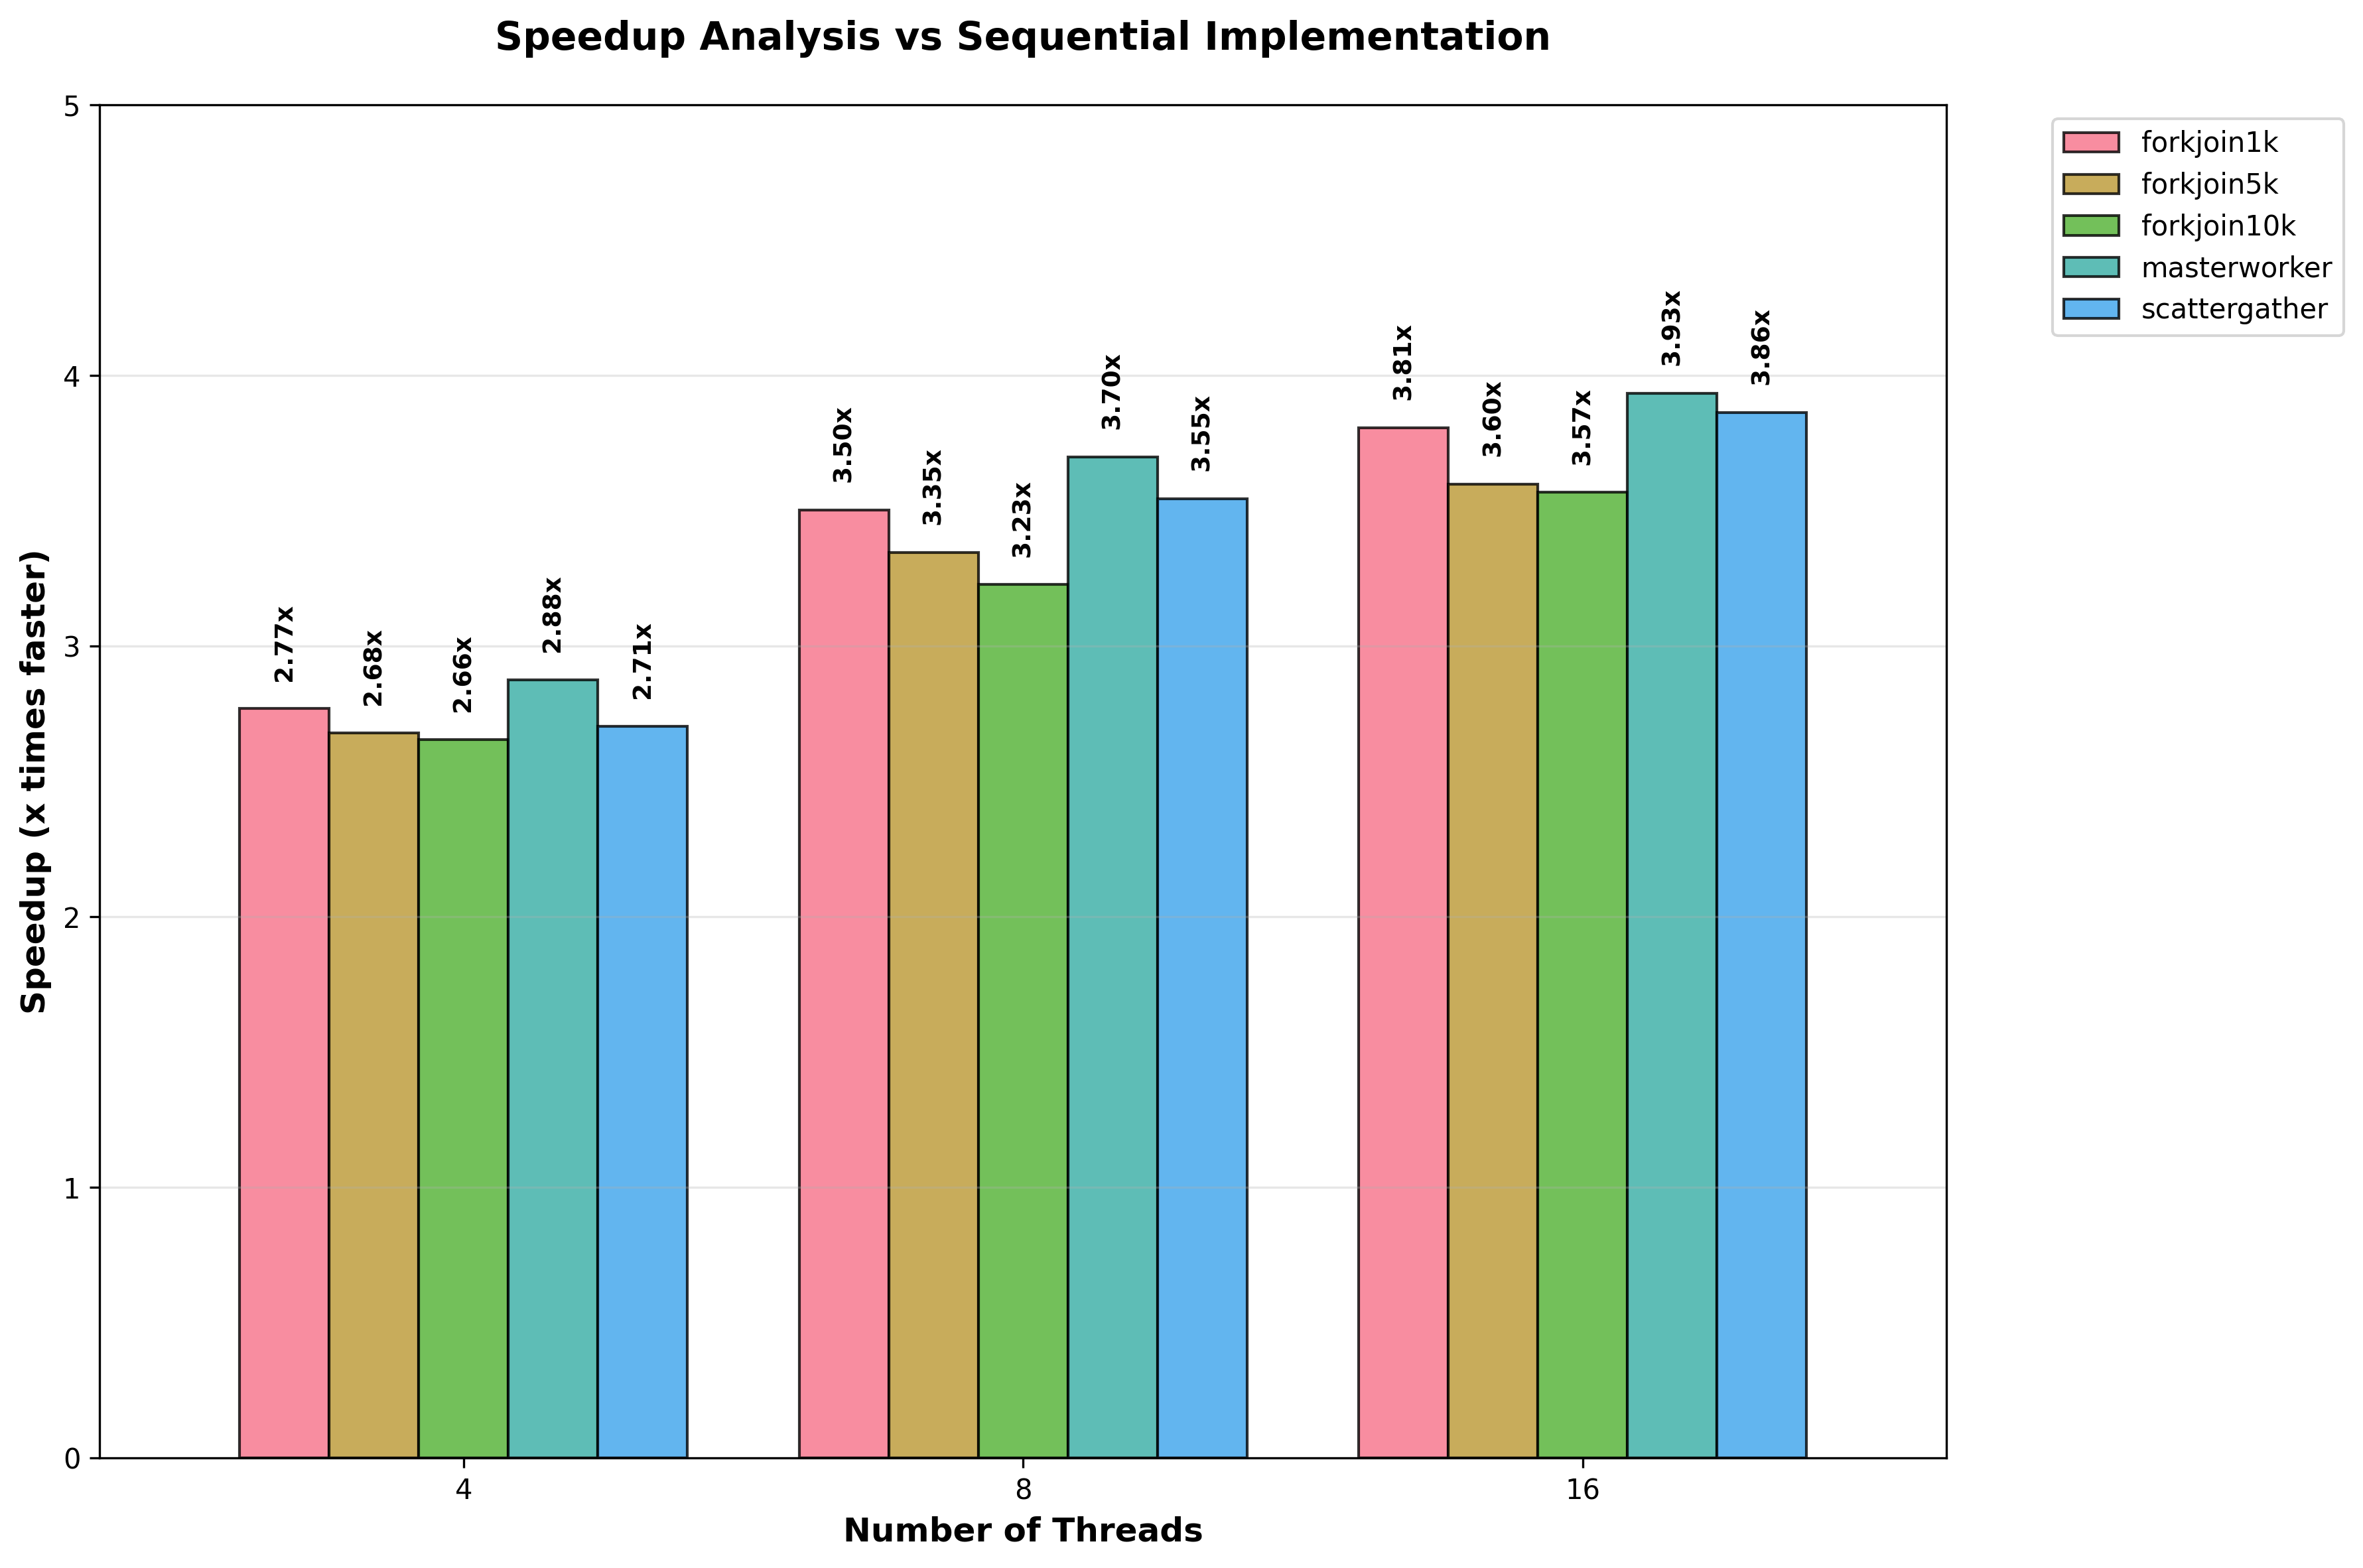
\includegraphics[width=\textwidth]{images/speedup_analysis.png}
    \caption{Speedup comparison across different parallel implementations}
    \label{fig:speedup}
\end{figure}

\begin{figure}[htbp]
   \centering
   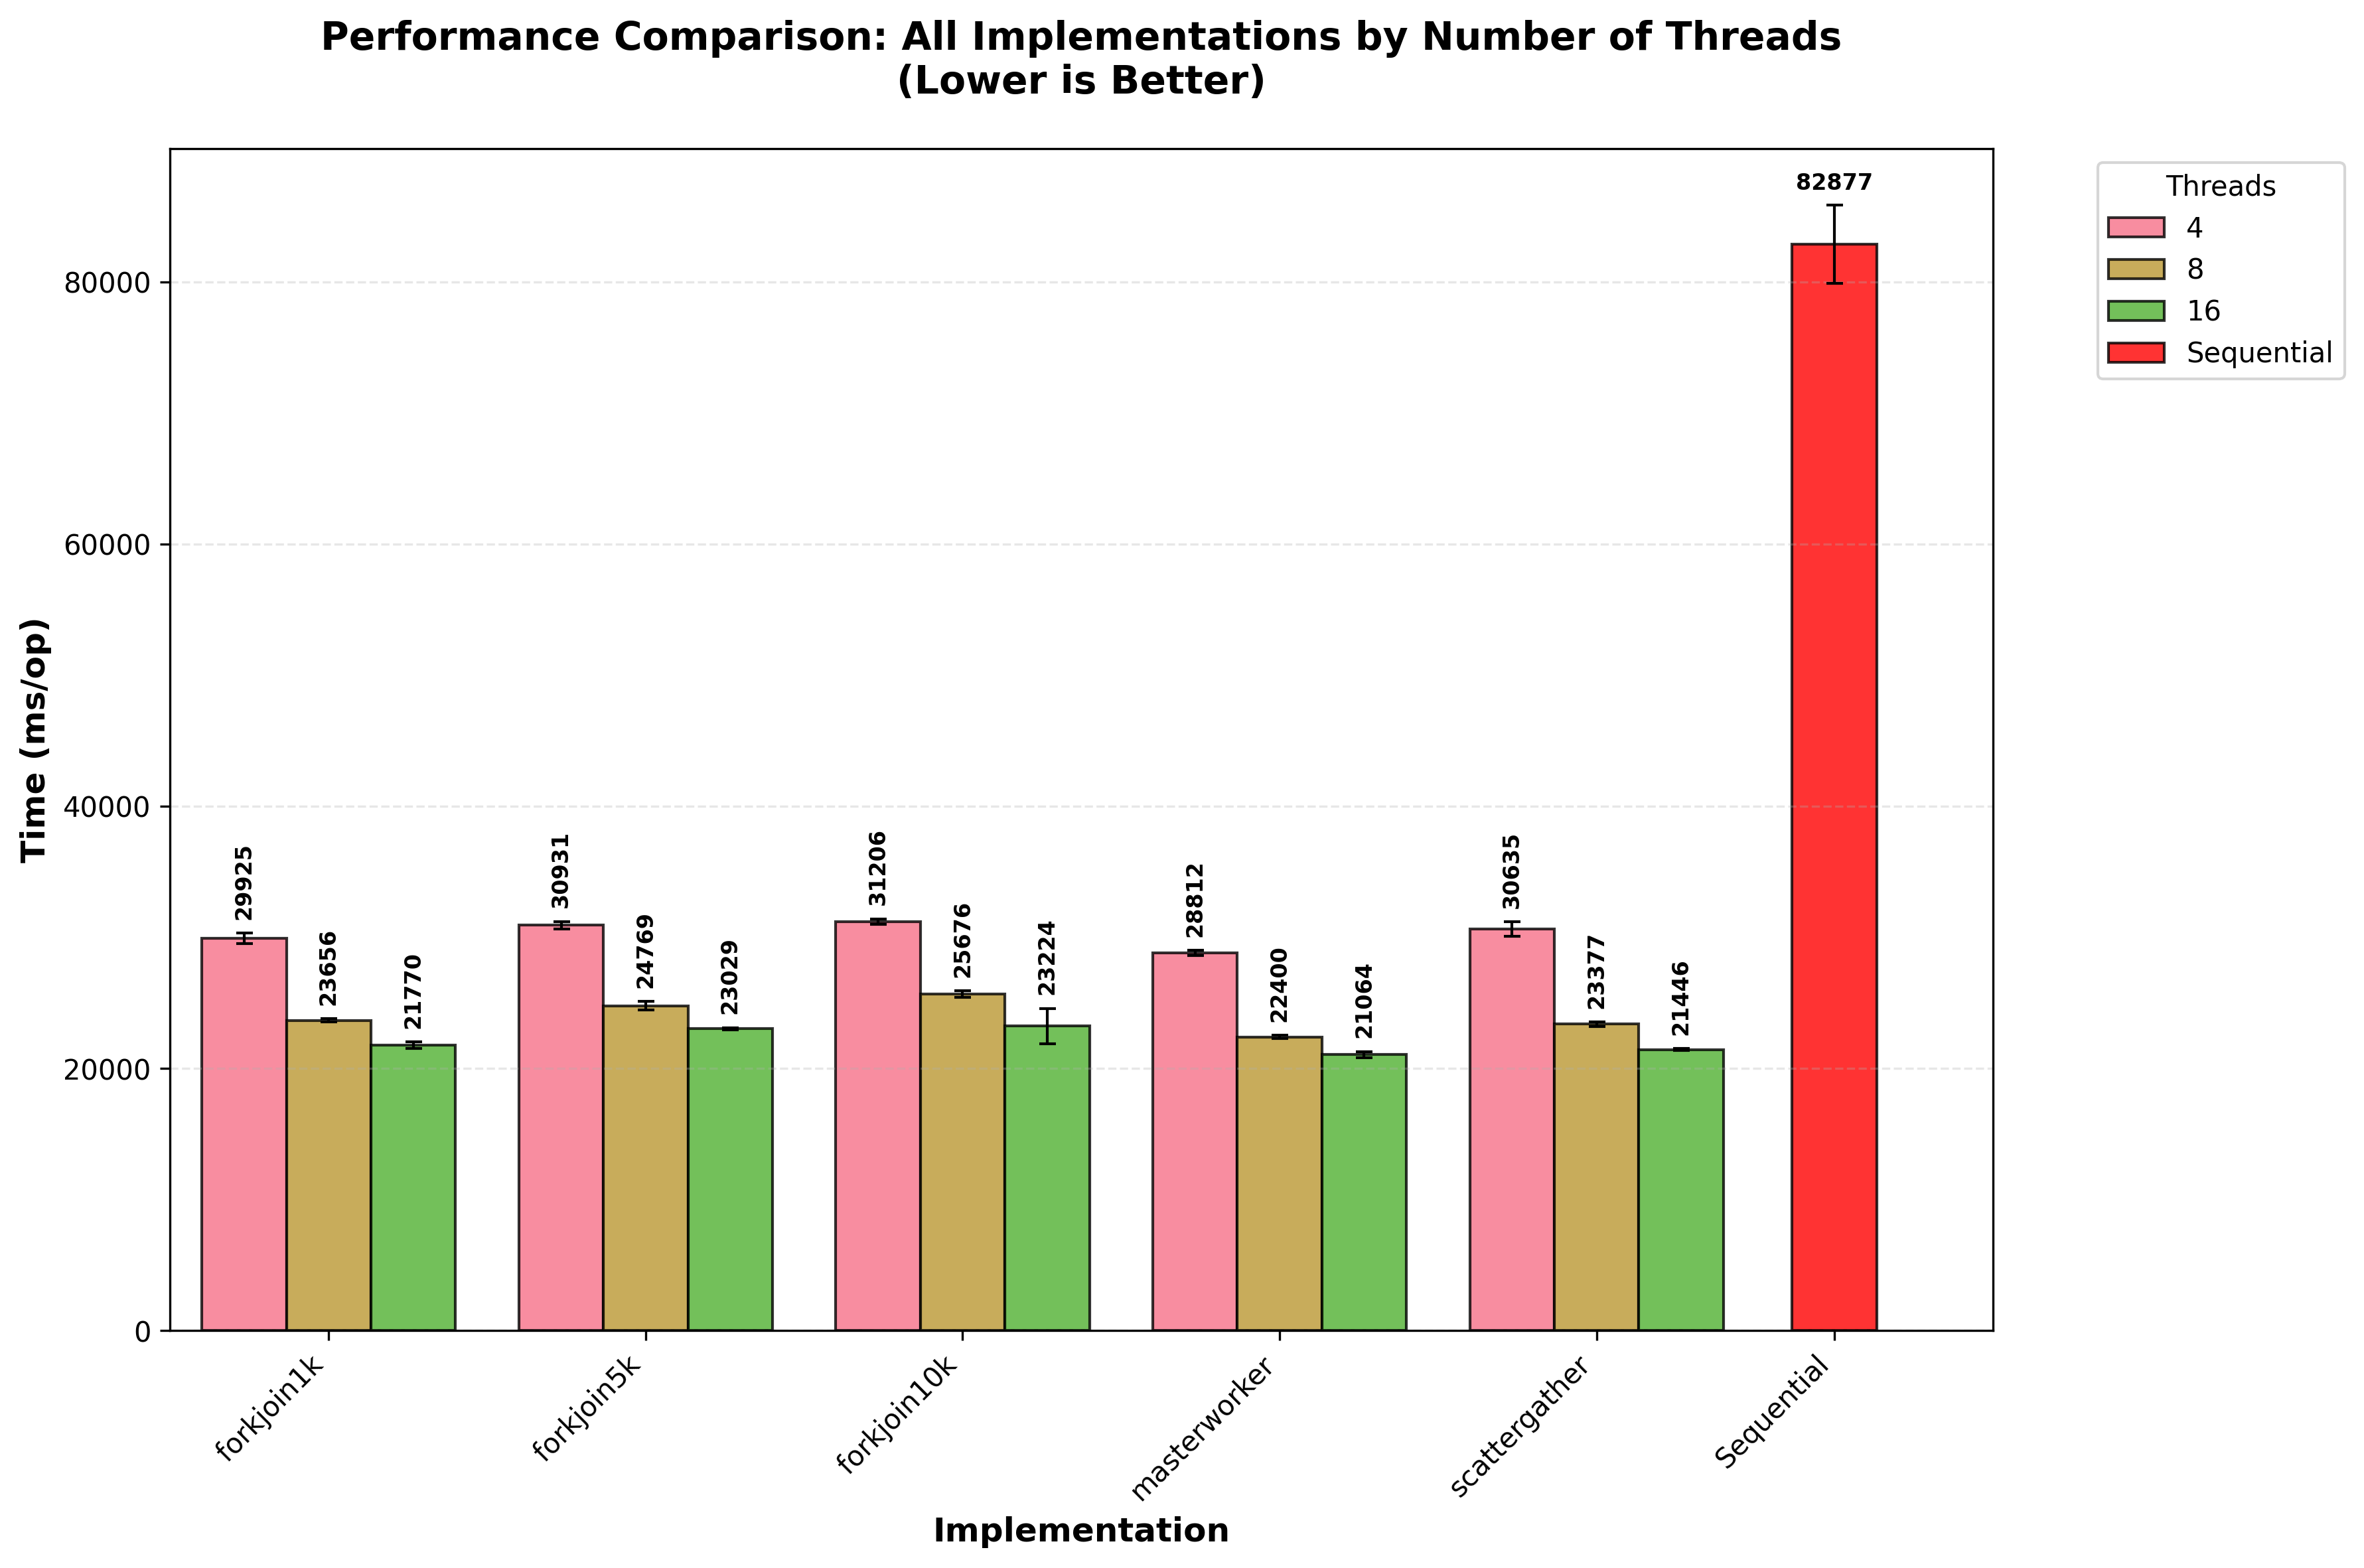
\includegraphics[width=\textwidth]{images/performance_comparison.png}
   \caption{Comprehensive performance comparison of all implementations}
   \label{fig:performance}
\end{figure}

\newpage

\section{Analysis of Performance Results}

The performance results can be explained by several key factors related to the
nature of the algorithm and the characteristics of each parallelization
strategy:

\subsection{Master-Worker Performance}

\begin{enumerate}
   \item \textbf{Configurable Worker Thread Pool}: This implementation creates
   workers equal to the \texttt{maxThreads} parameter that remain active
   throughout all generations, eliminating thread creation/destruction overhead
   \item \textbf{LinkedBlockingQueue Efficiency}: The thread-safe
   \texttt{LinkedBlockingQueue<Task>} provides optimal load balancing - workers
   continuously poll without spinning, and blocking ensures immediate task
   pickup
   \item \textbf{Poison Pill Termination}: The \texttt{TaskType.POISON\_PILL}
   shutdown mechanism in \texttt{stopWorkers()} minimizes synchronization
   complexity compared to other termination strategies
   \item \textbf{Chunked Population Processing}: Population division based on
   \texttt{POP\_SIZE / maxThreads} ensures consistent memory regions per worker,
   improving cache locality
   \item \textbf{CountDownLatch Synchronization}: Each operation uses precise
   synchronization barriers without unnecessary thread blocking between
   algorithm steps
\end{enumerate}

\newpage

\subsection{Fork-Join Threshold Analysis}

The threshold parameter significantly impacts performance across different
configurations:

\begin{enumerate}
   \item \textbf{1k Threshold Advantages}:
      \begin{itemize}
      \item Optimal task granularity for algorithm computational intensity
      \item Sufficient parallel tasks without excessive \texttt{RecursiveAction}
      creation overhead
      \item Effective work-stealing due to balanced task completion times
      \item Better utilization at high thread counts (16 threads)
      \end{itemize}

   \item \textbf{5k and 10k Threshold Limitations}:
      \begin{itemize}
      \item Larger chunks create fewer parallel opportunities, especially
      problematic at 16 threads
      \item Less effective work-stealing due to uneven task distribution
      \item Underutilization when chunk count $<$ available thread count
      \end{itemize}

   \item \textbf{Work-Stealing Framework}: The \texttt{ForkJoinPool} with
   \texttt{invokeAll()} provides automatic load balancing through work-stealing
   queues, explaining consistent scaling performance
\end{enumerate}

\subsection{Scatter-Gather Characteristics}

\begin{enumerate}
   \item \textbf{Configurable Thread Pool}:
   \texttt{Executors.newFixedThreadPool(maxThreads)} where \texttt{maxThreads}
   is a configurable parameter created once per execution minimizes thread
   management overhead across generations
   \item \textbf{Future-Based Coordination}: The \texttt{futures.forEach \{
   it.get() \}} pattern creates efficient synchronization barriers but requires
   all threads to complete before proceeding
   \item \textbf{Static Chunk Distribution}: Equal work distribution
   (\texttt{chunkSize = total operations / maxThreads}) works well for uniform
   algorithm workloads
\end{enumerate}

\newpage

\subsection{Efficiency}

\begin{figure}[htbp]
   \centering
   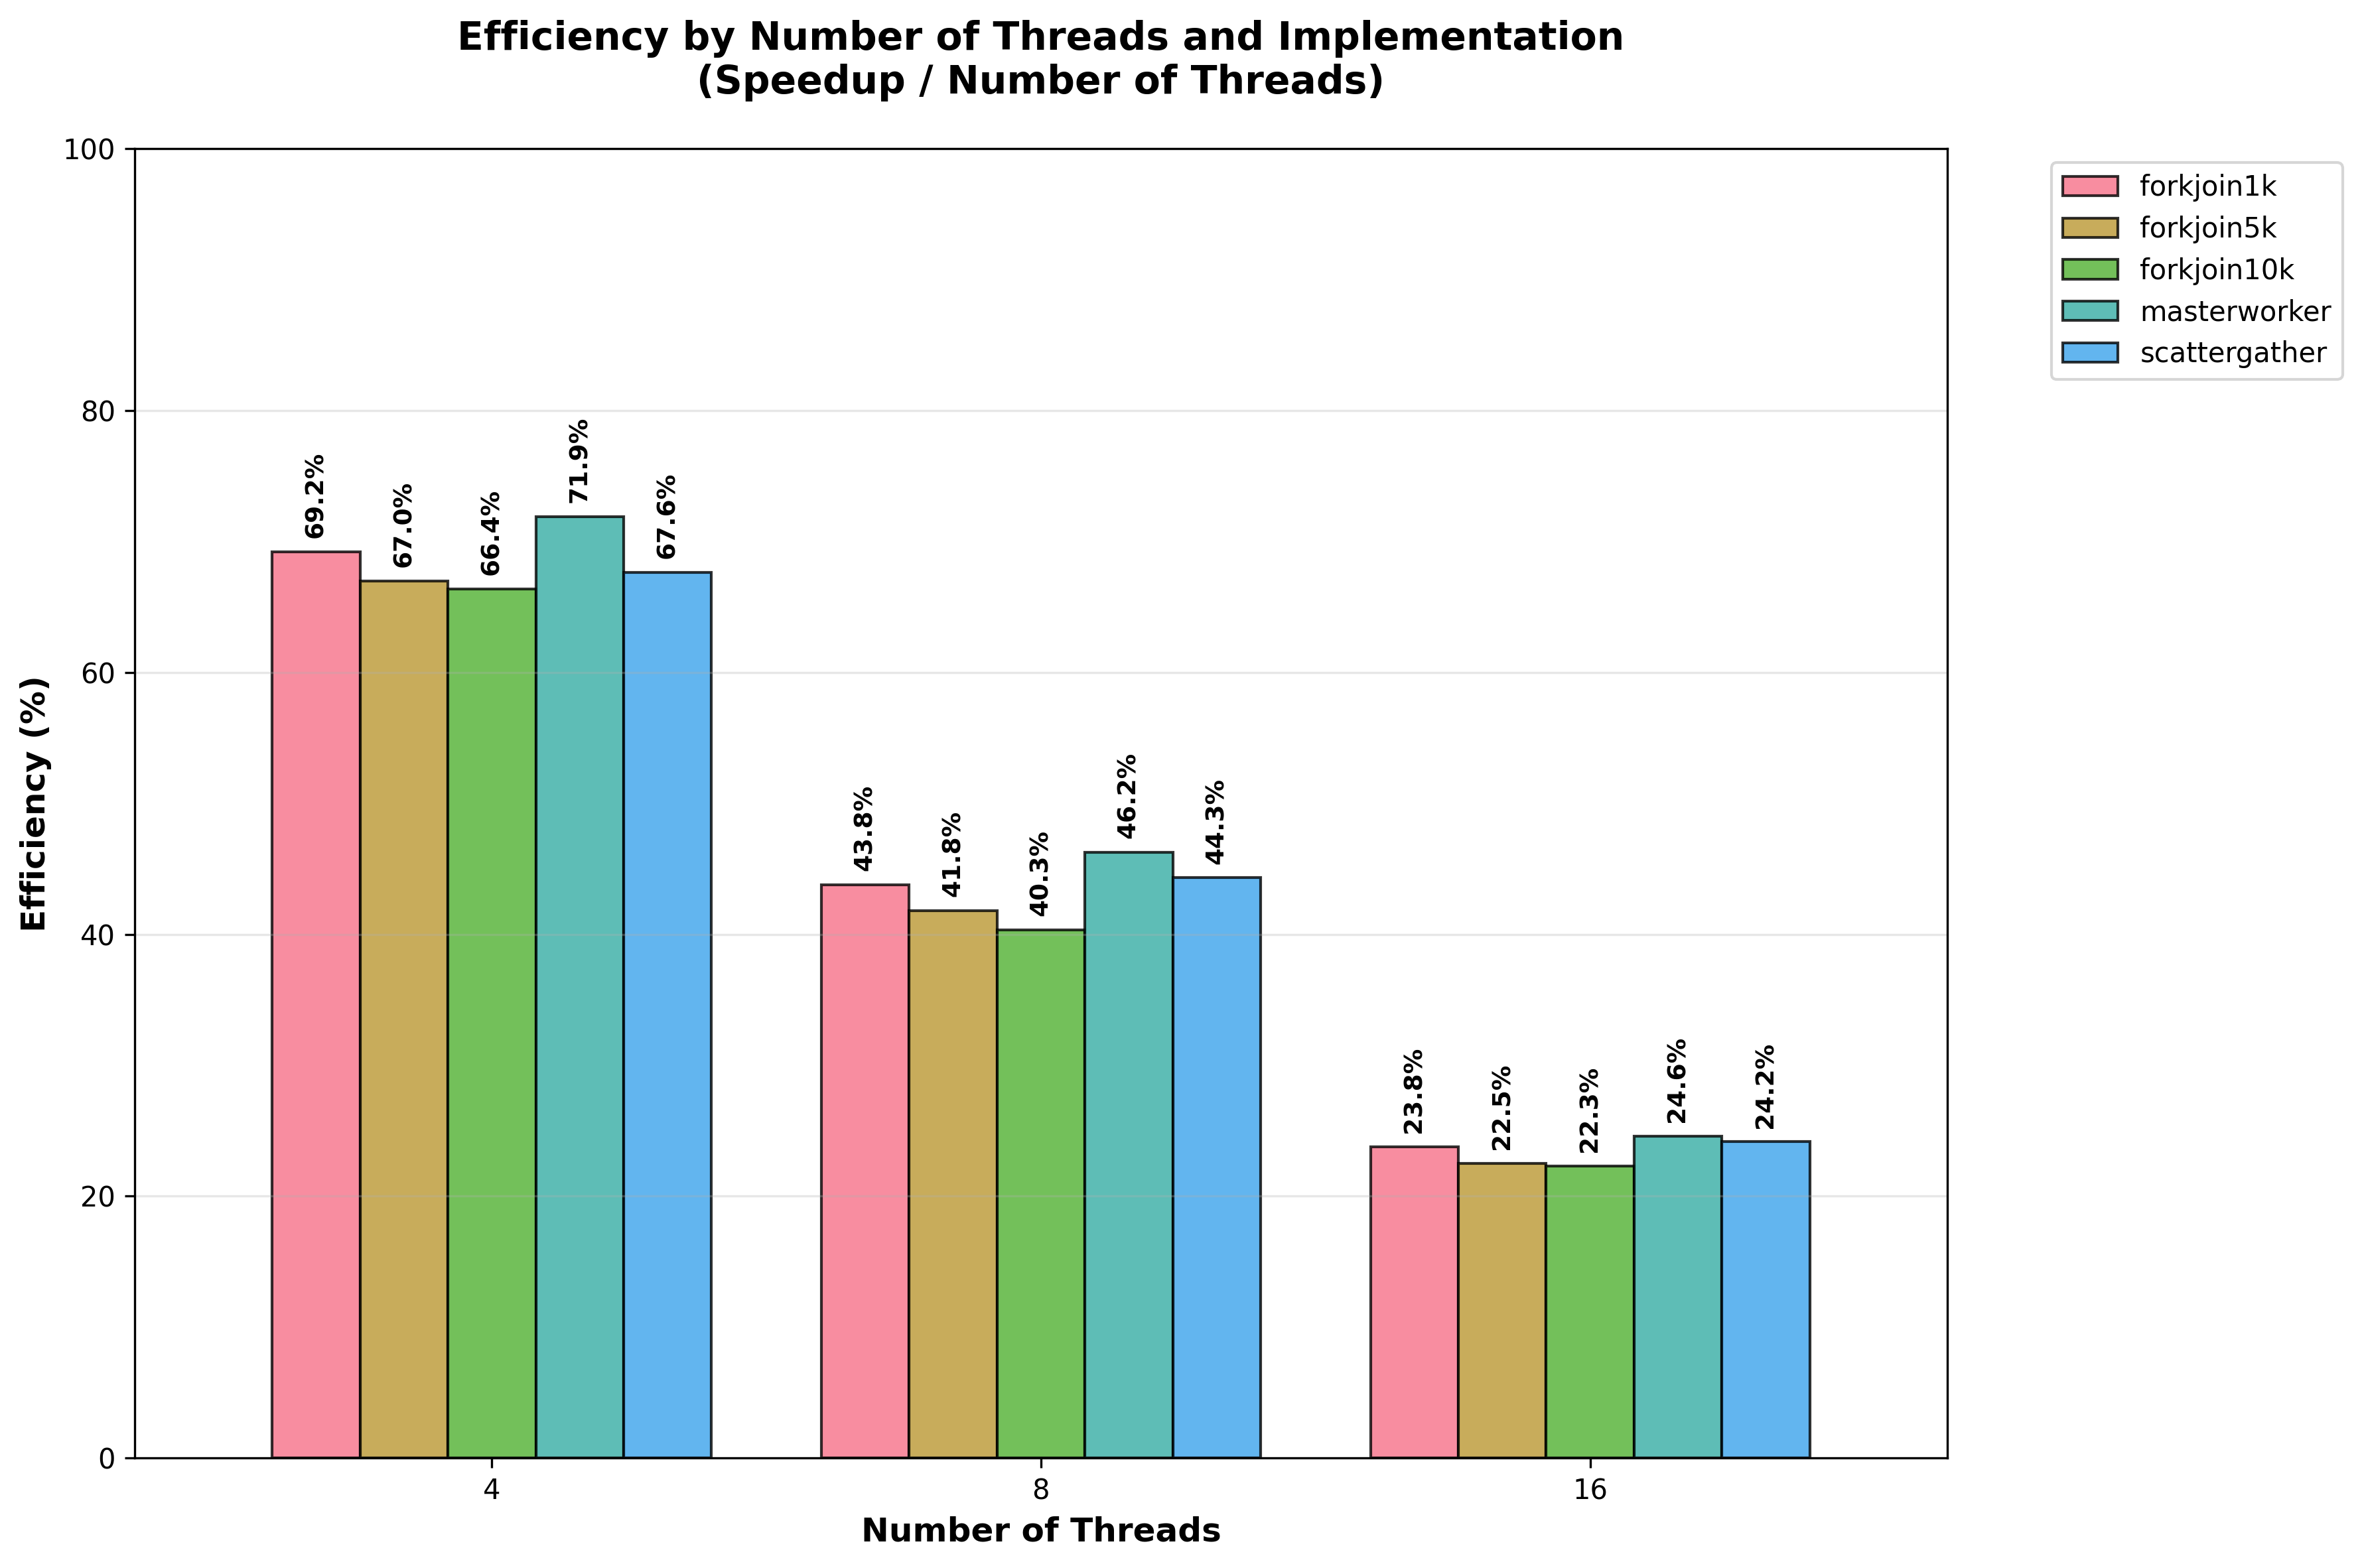
\includegraphics[width=0.7\textwidth]{images/efficiency_analysis.png}
   \caption{Efficiency analysis for various thread counts}
   \label{fig:efficiency}
\end{figure}

The efficiency follows fundamental parallel computing limitations:

\begin{enumerate}
   \item \textbf{Amdahl's Law}: Sequential algorithm portions (initialization,
   result collection, synchronization points) become bottlenecks as parallel
   portions accelerate
   \item \textbf{Synchronization Overhead Scaling}:
   \texttt{CountDownLatch.await()} and \texttt{AtomicReference} compare-and-swap
   operations become more expensive with increased thread contention
   \item \textbf{Memory Subsystem Saturation}:
      \begin{itemize}
      \item Cache consistency overhead increases with thread count
      \item Memory bandwidth limits during population array manipulation
      \item Potential false sharing in population data structures
      \end{itemize}
   \item \textbf{Hardware Architecture Limits}: Beyond 8 threads, hyperthreading
   effects significantly reduce per-thread effectiveness since the experimental
   setup uses a machine with 8 physical cores and 16 logical processors
   (hyperthreading enabled). Threads 9-16 share execution units, caches, and
   pipeline resources with threads 1-8, leading to resource contention rather
   than true parallelism
\end{enumerate}

\subsection{Implementation-Specific Performance Factors}

\begin{itemize}
   \item \textbf{Master-Worker}: Persistent threads + efficient task queue =
   minimal coordination overhead
   \item \textbf{Fork-Join 1k}: Optimal granularity + recursive work-stealing =
   superior load balancing
   \item \textbf{Scatter-Gather}: Simple coordination + thread pool reuse =
   solid baseline performance
   \item \textbf{Fork-Join 5k/10k}: Suboptimal granularity limits
   parallelization effectiveness at higher thread counts
\end{itemize}

\subsection{Experimental Setup}
The experimental setup for evaluating the performance of the algorithm
implementations involved the following key components:

\begin{itemize}
   \item \textbf{Hardware}: The machine used for testing is equipped with an AMD
   Ryzen 7 processor featuring 8 physical cores and 16 logical processors
   (hyperthreading enabled), along with 16GB of RAM. This configuration allows
   for testing various thread counts up to 16.
   \item \textbf{Operating System}: The experiments were conducted on a 64-bit
   version of Windows 11.
   \item \textbf{Java Version}: All implementations were developed and executed
   using OpenJDK 17.0.16+8.
   \item \textbf{Benchmarking Framework}: The JMH (Java Microbenchmark Harness)
   was used to ensure accurate and reliable performance measurements using the
   following configurations for the parallel implementations:
   \begin{itemize}
   \item Benchmark mode: Average time
   \item Output time unit: milliseconds
   \item Forks: 3
   \item Warm-up iterations: 3 with 2 seconds each
   \item Measurement iterations: 5 with 2 seconds each
   \end{itemize}
\end{itemize}

\chapter{Conclusions} \label{cap:conclusions}

In this assignment successfully demonstrated the effectiveness of parallel
algorithms for the knapsack problem, achieving significant speedups ranging from
\textbf{2.6x to 3.9x} compared to sequential implementation. The Master-Worker
pattern emerged as the optimal approach (3.93x speedup at 16 threads) due to its
efficient thread lifecycle management and task distribution via
\texttt{LinkedBlockingQueue} with poison pill termination.

The results confirm that algorithms are well-suited for parallelization, with
fitness evaluation being an embarrassingly parallel operation. However,
efficiency diminishes with increased thread count (72\% at 4 threads to 25\% at
16 threads) due to hyperthreading effects, synchronization overhead, and memory
subsystem limitations beyond 8 physical cores.

  

% \bibliographystyle{unsrt} \bibliography{referencias}
% \addcontentsline{toc}{chapter}{References}

% % Apêndices (opcional) \appendix \include{appendix}

\end{document} 